%% Einleitung.tex
%% $Id: einleitung.tex 61 2012-05-03 13:58:03Z bless $
%%

\chapter{Einleitung}
\label{ch:Einleitung}
%% ==============================
Die Einleitung besteht aus der Motivation, der Problemstellung, der Zielsetzung und einem erster Überblick über den Aufbau der Arbeit.

%% ==============================
\section{Motivation}
%% ==============================
\label{ch:Einleitung:sec:Motivation}
Das \emph{Knotenüberdeckungsproblem}, oder englisch Vertex Cover, ist ein nachgewiesen NP-vollständiges Problem \cite{intract}, kann also von einem nichtdeterministischen Algorithmus in Polinomialzeit gelöst werden. Um das Problem zu erklären, betrachten wir ein Netz von Haushalten, bei dem wir die Möglichkeit haben, in jedem Haushalt einen Stromgenerator zu platzieren, sodass durch alle mit diesem Haus verbundenen Leitungen Strom fließt. Ziel ist, ein stabiles Stromnetz zu schaffen, bei dem jede Leitung an mindestens eine Stromquelle angeschlossen ist. Nun ergibt sich das Problem, dass die Kosten für Stromgeneratoren erheblich sind und daher nur maximal \emph{k} Geräte angeschafft werden können. Es gilt also, aus den \emph{n} Häusern \emph{k} oder weniger auszuwählen, sodass jede Leitung von einem der Häuser in der Auswahl versorgt wird.
\begin{figure}[htb]
\centering
  	{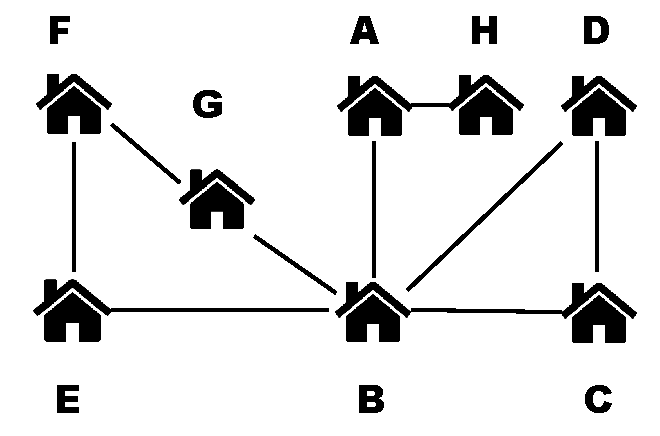
\includegraphics[width=.5\textwidth]{vertexcoverBsp.pdf}}
	\caption{Graph eines Stromnetzes \label{fig:vc}}
\centering
\end{figure}
In Abbildung \ref{fig:vc}\footnote{Icons in der Graphik von https://www.flaticon.com/}   sieht man ein Beispiel für eine solche Probleminstanz. Die Haushalte sind jeweils mit einem Buchstaben gekennzeichnet; jede Linie, beziehungsweise Kante eine Leitung zum Nachbarhaus. Hier ist es möglich eine Lösung für \emph{k} = 4 zu finden, also 4 Häuser mit Generatoren auszustatten, sodass alle Leitungen versorgt sind. Bei einem kleinen Beispiel, wie hier ist zum Beispiel durch ausprobieren leicht zu sehen, dass es keine Lösung mit weniger Häusern, beziehungsweise Generatoren gibt. Um 4 Häuser, die das Problem lösen zu finden, könnten alle Möglichkeiten ausprobiert werden. Ein solcher naiver Algorithmus würde eine Laufzeit von $O(n^{k} \cdot m)$ ($m$ = Anzahl der Leitungen) brauchen, da für jede $k$ große Kombination aus Häusern, die Versorgung der Leitungen überprüft werden muss.\\
Mit einem einfachen Suchbaumalgorithmus betrachtet man jede Leitung nur einmal und entscheidet, welches der beiden Häuser mit einem Generator versorgt werden soll, da mindestens eins der beiden Häuser in der Lösungsmenge ist. Dadurch ergibt sich für jede Entscheindung eine Verzweigung. Nach $k$ Verzweigungen sind dann $k$ Generatoren verteilt und es muss überprüft werden, ob jede Leitung versorgt ist, was wiederum in $m$ Schritten gemacht werden kann. Es ergibt sich eine Laufzeit von $O(2^{k}) \cdot m$.
Nach der Verwendung eines dieser Algroithmen, finden sich die Lösung, dass wenn die Haushalte F, B, A und C oder F, B, A und D mit einem Generator ausgestattet werden, durch alle Leitungen Strom fließt. Für eine Problemgröße wie sie hier geschildert wird, bieten diese Mehtoden eine Lösung. Für eine Häusermenge \emph{n} = 2000 mit entsprechend vielen Leitungen bedeutet das ungefähr $1.148 \cdot 10^{602}$ mögliche Kombinationen.

Es ist leicht zu sehen, dass sich das Stromnetzproblem, ersetzt man die Häuser durch Knoten eines Graphen und die Leitungen durch dessen Kanten, zum Knotenüberdeckungsproblem transformieren lässt. Zu diesem Problem lassen sich zwei Fragestellungen unterscheiden: Zum Einen das Finden einer minimalen Knotenüberdeckung \cite{trees}:
\begin{align*}
EINGABE: &\ Graph\ G=(V,E),\ positive\ Integer\ k\leq |V|\\
AUSGABE: &\ S\subseteq V\ mit\ |S|\leq k,\\
&\ sodass\ jede\ Kante\ aus\ E\ einen\ Endpunkt\ in\ S\ hat.
\end{align*}
Zum Anderen das Entscheidungsproblem, ob es eine Knotenüberdeckung einer Größe $\leq k$ gibt:
\begin{align*}
EINGABE: &\ Graph\ G=(V,E),\ positive\ Integer\ k\leq |V|\\
AUSGABE: &\textit{Existiert ein}\ S\subseteq V\ mit\ |S|\leq k,\\
&\ sodass\ jede\ Kante\ aus\ E\ einen\ Endpunkt\ in\ S\ hat.
\end{align*}
Letzteres ist in der Liste von Karps 21 NP-vollständigen Problemen zu finden \cite{karp}.
Es existieren weitere reale Probleme, für die das Knotenüberdeckungsproblem anwendbar ist. Abu-Khzam et al \cite{paper:3} schlagen eine Anwendung in der Bioinformatik vor.
Ein nichtdeterministischer Algorithmus kann jede vermeintliche Lösungskombination aus Knoten, beziehzungsweise Haushalten in Polynomialzeit testen \cite{intract}, da lediglich überprüft werden muss, ob die Größe der Lösungsmenge den Wert von \emph{k} überschreitet und ob alle Kanten abgedeckt (Leitungen versorgt) sind.
 Allerdings würde ein naiver Algrithmus für große Eingaben in der Realität nicht in absehbarer Zeit terminieren, wie beispielhaft in Tabelle \ref{tab:exponential} zu sehen ist.
 
 \begin{table}[htb]
\caption{Exponentielle Laufzeit \label{tab:exponential}}
\vspace*{1em}
\centering

\bgroup
\def\arraystretch{1.3}%  1 is the default, change whatever you need

\begin{threeparttable}

\begin{tabular}[c]{ l | l }
	
	\multicolumn{1}{c|}{\textbf{Eingabegröße}} & 
	\multicolumn{1}{c}{\textbf{Laufzeit}} \\ 
	
	\hline

	$2^{1}$& 0.00002s\\
	$2^{10}$& 0.02s\\
	$2^{100}$& ca. $ 2 \cdot 10^{14} $ Jahrtausende \\
	
\end{tabular}

\begin{tablenotes}\footnotesize
\item EINFÜGEN
\end{tablenotes}

\end{threeparttable}

\egroup

\end{table}
Es ist also sinnvoll, die Eingabe möglichst klein zu halten und zu \emph{reduzieren}, indem einfache Teile des Graphen durch Vorverarbeitung, englisch \emph{Preprocessing}, entfernt werden und gegebenenfalls in die Lösungsmenge aufgenommen werden, Die sollte in Polinomialzeit geschehen, um die gesamte Laufzeit zu reduzieren. Das Ziel der in dieser Arbeit verwendeten Reduktionsregeln ist für einen gegebenen Graphen $G=(V,E)$ und einer natürlichen Zahl $k$ und der Problemstellung $VC(G,k)$ das Finden und Entfernen eines induzierten Teilgraphen $G' \subseteq G$ und Verkleinerung von $k$
sodass für den Problemkern $G'' = G \setminus G'$ gilt, dass $VC(G,k) = VC(G'',k'') \cup C\ mit\ C=VC(G', k'')$, wobei $C=VC(G', k'')$ in Polinomialzeit durch die Regeln berechnen lässt. Für den Suchbaumalgorithmus (mit $O(2^{k} \cdot m)$) bedeutet jede Reduzierung von $k$ eine Verdoppelung der Geschwindigkeit. 


%% ==============================
\section{Problemstellung}
%% ==============================
\label{ch:Einleitung:sec:Problemstellung}

Das Knotenüberdeckungsproblem ist in der Literatur viel vertreten und es wurden verschiedene Reduktionsregeln entdeckt. In dieser Arbeit werden einfachere Reduktionsregeln, genauer gesagt die Grad$_{0}$-, Grad$_{1}$- und Buss-Regel betrachtet, als auch Nemhauser-Trotter-Regel und Kronenregel, welche sich weitaus komplexer gestalten. Jede Regel greift an verschiedenen Stellen eines Graphen und es scheint, dass die Reihenfolge, in der verschiedene Regeln auf einen Graphen angewandt werden einen Einfluss auf die insgesamt erreichte Reduktion hat. In dieser Arbeit wird untersucht, wie sich verschiedene Regeln in der Praxis verhalten, sowohl einzeln als auch in Kombination, und verglichen. 

%% ==============================
\section{Zielsetzung}
%% ==============================
\label{ch:Einleitung:sec:Zielsetzung}

Ein Großteil der Behandlung von Reduktionsregeln in der Literatur findet ausschließlich theoretisch statt.
Ziel dieser Arbeit ist, herauszufinden, wie sich die Regeln in der Praxis verhalten, wenn sie einzeln oder in Kombination miteinander angewandt werden. Hierzu wurden die Regeln mithilfe der C++-Library LEDA \cite{manual} implementiert, welche Algorithmen und eingene Datentypen bereitstellt. Unter anderem liefert LEDA Datenstrukturen für Graphen, Algorithmen für Graphen, wie zum Beispiel eine Funktion, mit der ein Maximum-Bipartite-Matching in einem Graphen gefunden und ausgegeben wird. Durch die Vielzahl an Funktionen eignet sich die Library für diese Arbeit. Jede Regel wird dann unter verschiedenen Aspekten untersucht:
\begin{itemize}
\item Wie verhält sich die die theoretische Laufzeit im Vergleich zur Praxisanwendung?
\item Passt die theoretisch erwartete Reduktion zum Ergebnis am Testset?
\item Wie gut ist das Ergebnis der Reduktion im Vergleich zu anderen Regeln?
\item Welche Kombination von Regeln liefert eine hohe/niedrige Reduktion? Warum?
\item Wie sehen Graphen aus, auf die keine Regel anwendbar ist?
\item Wie sehen Graphen aus, auf die genau eine Regel anwendbar ist?
\end{itemize}


%% ==============================
\section{Gliederung der Arbeit}
%% ==============================
\label{ch:Einleitung:sec:Gliederung}

Zunächst werden einige Grundlagen geschaffen, um auf gewisse Begrifflichkeiten in späteren Kapiteln zurückgreifen zu können, um dann die entsprechenden Algorithmen vorzustellen. Kapitel \ref{ch:Analyse} beschäftigt sich mit der Analyse der Praxisanwendung der Regeln und zeigt mögliche Gründe für die gefundenen Ergebnisse. Im folgenden Kapitel wird auf Besonderheiten in der Implementierung und Umsetung der Reduktionsregeln eingegangen, um abschließend im Fazit einen Ausblick auf mögliche zukünftige Problemstellungen zu geben.






%%% Local Variables: 
%%% mode: latex
%%% TeX-master: "thesis"
%%% End: 
